En la carpeta \texttt{mediciones} se encuentran los archivos de salida correspondientes a cada
experimento. Por cada uno, se adjunta un archivo \texttt{README.txt} con la información conocida
sobre la red en cuestión y otro arhivo \texttt{exceptions.txt} que describe los paquetes sin tipo
capturados. Los nombres de los experimentos denotan el tipo de red, el tipo de conexión y la
duración del experimento en minutos.

\subsubsection{Experimento 1: Red hogareña, cableada, 10 mintos (\texttt{home-eth-10})}

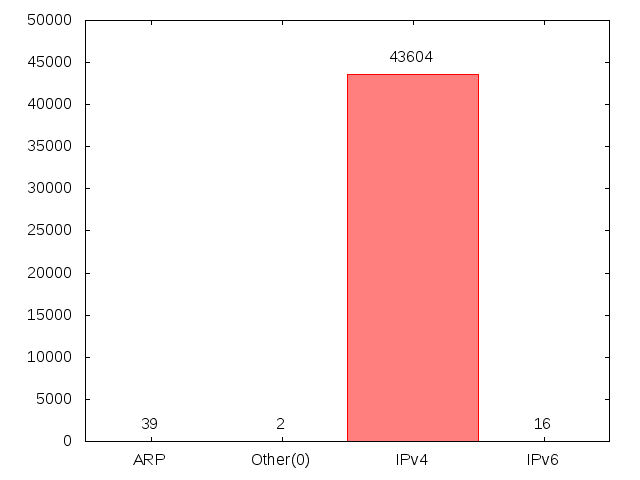
\includegraphics{../mediciones/home-eth-10/home-eth-10Protocolos.png}
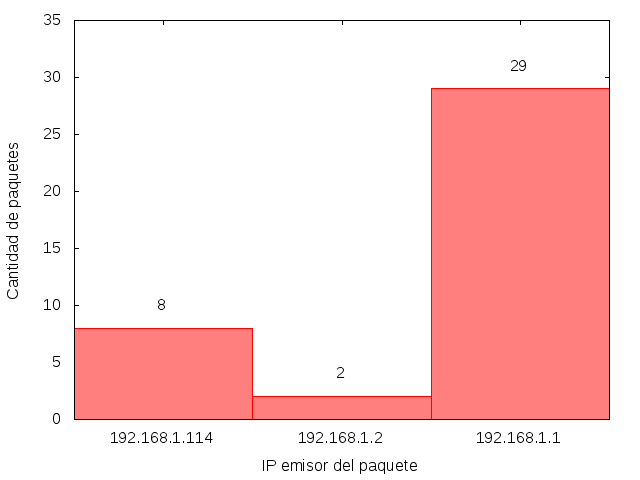
\includegraphics{../mediciones/home-eth-10/home-eth-10IpsSrcArp.png}
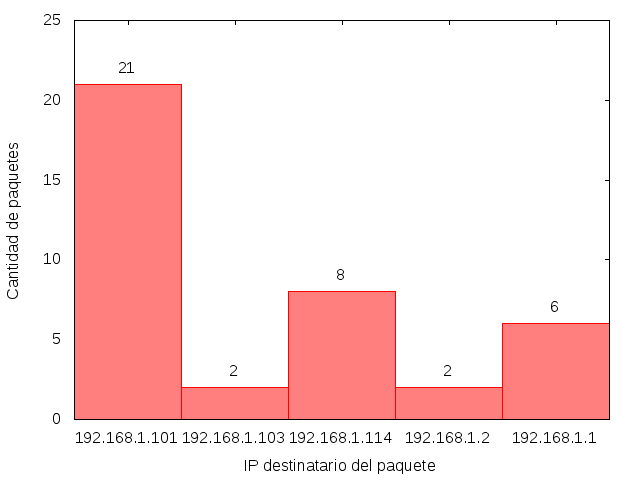
\includegraphics{../mediciones/home-eth-10/home-eth-10IpsDstArp.png}

\subsubsection{Experimento 1: Red hogareña, inalámbrica, 10 mintos (\texttt{home-wfi-10})}

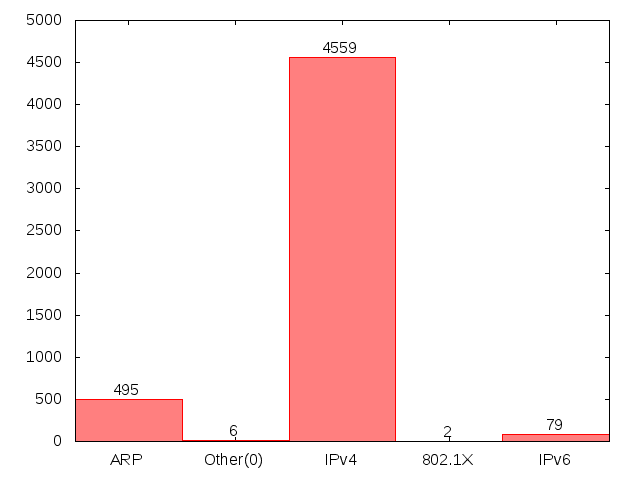
\includegraphics{../mediciones/home-wfi-10/home-wfi-10Protocolos.png}
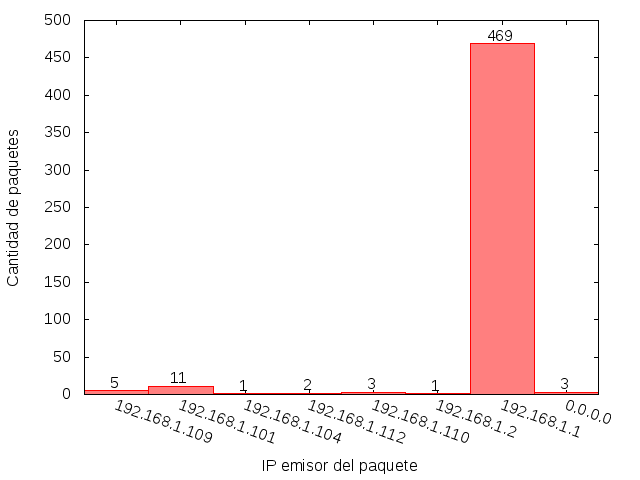
\includegraphics{../mediciones/home-wfi-10/home-wfi-10IpsSrcArp.png}
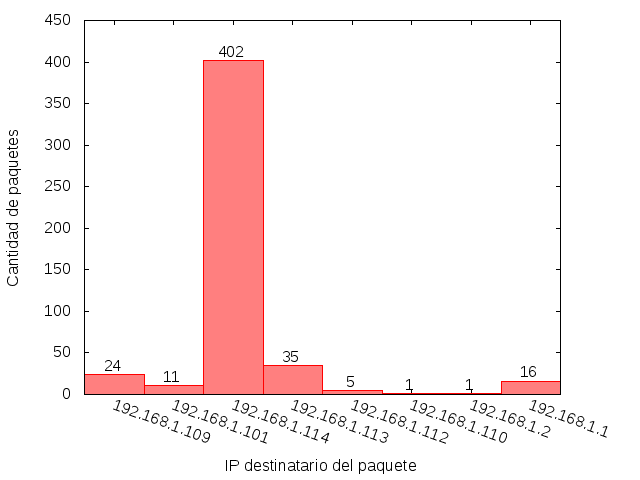
\includegraphics{../mediciones/home-wfi-10/home-wfi-10IpsDstArp.png}
